% Publication-Grade Causal DAG: Instrumental Variable Design
% Adheres to Angrist, Imbens, and Rubin (1996) and Pearl (2009)
% Compile with pdflatex or lualatex

\documentclass[tikz,border=10pt]{standalone}
\usepackage{tikz}
\usetikzlibrary{arrows.meta,positioning,shapes.geometric}

\begin{document}
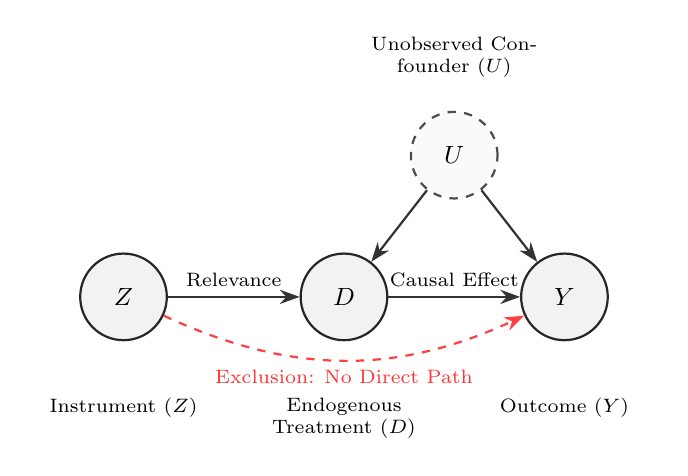
\begin{tikzpicture}[
    node distance=2.2cm and 2.5cm,
    every node/.style={font=\sffamily\small},
    observed/.style={circle, draw=black!85, fill=black!5, thick, minimum size=1.1cm},
    unobserved/.style={circle, draw=black!70, dashed, fill=black!2, thick, minimum size=1.1cm},
    edge/.style={->, >={Stealth[length=2.5mm, width=1.8mm]}, thick, draw=black!80},
    forbidden/.style={->, >={Stealth[length=2.5mm, width=1.8mm]}, thick, dashed, draw=red!75}
]

    % Nodes
    \node[observed] (Z) at (0, 0) {$Z$};
    \node[observed] (D) at (2.8, 0) {$D$};
    \node[observed] (Y) at (5.6, 0) {$Y$};
    \node[unobserved] (U) at (4.2, 1.8) {$U$};

    % Direct arrows
    \draw[edge] (Z) -- node[above, font=\scriptsize] {Relevance} (D);
    \draw[edge] (D) -- node[above, font=\scriptsize] {Causal Effect} (Y);
    \draw[edge] (U) -- (D);
    \draw[edge] (U) -- (Y);

    % Excluded path (forbidden by exclusion restriction)
    \draw[forbidden] (Z) to[bend right=25] node[below, font=\scriptsize, text=red!80] {Exclusion: No Direct Path} (Y);

    % Node labels
    \node[below=0.6cm of Z, text width=2.2cm, align=center, font=\scriptsize] {Instrument ($Z$)};
    \node[below=0.6cm of D, text width=2.2cm, align=center, font=\scriptsize] {Endogenous Treatment ($D$)};
    \node[below=0.6cm of Y, text width=2.2cm, align=center, font=\scriptsize] {Outcome ($Y$)};
    \node[above=0.3cm of U, text width=3.0cm, align=center, font=\scriptsize] {Unobserved Confounder ($U$)};

\end{tikzpicture}
\end{document}
